\documentclass[border=2pt, 12pt]{standalone}

\usepackage[dvipsnames]{xcolor}
    \definecolor{GDLcolor}{HTML}{a6a6a6}
    \definecolor{ELcolor}{HTML}{f3f1c5}

\usepackage{tikz}
    \usetikzlibrary{math}

\begin{document}
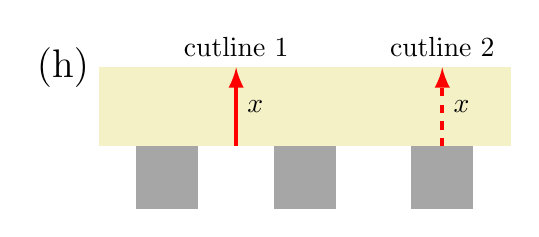
\begin{tikzpicture}
    \tikzmath{%
        \dpore=0.96;
        \epsilonGDL=0.55;
        \deltawall=(1-\epsilonGDL)*\dpore/\epsilonGDL;
        \deltafig=3*\dpore+3*\deltawall;
        \deltaEL=1;
    };

    \fill [ELcolor] (0, 0) rectangle (\deltafig, \deltaEL);
    \foreach \i in {0, ..., 2} {%
            \fill [GDLcolor] ({\dpore/2+\i*(\deltawall+\dpore)}, 0) rectangle ++(\deltawall, -0.8*\deltaEL);
        }

    % y
%    \draw [-latex, red, line width=1.5pt] (0, 0) -- ++(\deltafig, 0);
%    \node [above] at (\dpore/2+\deltawall/2, 0) {$ y $};
%    \node [left] at (0, \deltaEL) {\fontsize{14pt}{14pt}\selectfont (g)};

    % x
        \draw [-latex, red, line width=1.5pt] (\dpore+\deltawall, 0) -- ++(0, \deltaEL)
        node [pos=0.5, right, black] {$ x $}
        node [above, black] {cutline 1};
        \draw [-latex, red, dashed, line width=1.5pt] (2.5*\dpore+2.5*\deltawall, 0) -- ++(0, \deltaEL)
        node [pos=0.5, right, black] {$ x $}
        node [above, black] {cutline 2};
        \node [left] at (0, \deltaEL) {\fontsize{14pt}{14pt}\selectfont (h)};

\end{tikzpicture}
\end{document}